\documentclass{chi2009}
\usepackage{times}
\usepackage{url}
\usepackage{graphics}
\usepackage{color}
\usepackage[pdftex]{hyperref}
\hypersetup{%
pdftitle={TwinList: \\ Visualizing List Differences},
pdfauthor={Leonardo Max Baptista Claudino, claudino@cs.umd.edu \\
	    Sameh Khamis, sameh@cs.umd.edu \\
	    Ran Liu, ranliu@cs.umd.edu \\
	    Ben London, blondon@cs.umd.edu \\
	    Jay Pujara, jay@cs.umd.edu},
pdfkeywords={list visualization},
bookmarksnumbered,
pdfstartview={FitH},
colorlinks,
citecolor=black,
filecolor=black,
linkcolor=black,
urlcolor=black,
breaklinks=true,
}
\newcommand{\comment}[1]{}
\definecolor{Orange}{rgb}{1,0.5,0}
\newcommand{\todo}[1]{\textsf{\textbf{\textcolor{Orange}{[[#1]]}}}}

% TwinList Macros
\newcommand{\TwinList}{\textsc{TwinList}}
\newcommand{\ListViewer}{\textit{List Viewer}}
\newcommand{\AcceptReject}{\textit{Accept/Reject}}
\newcommand{\AcceptedRejected}{\textit{Accepted/Rejected}}
\newcommand{\Details}{\textit{Details Panel}}
\newcommand{\Tools}{\textit{Tools Dock}}
\newcommand{\Controls}{\textit{Control Panel}}
\newcommand{\Filters}{\textit{Filter Panel}}
\newcommand{\Options}{\textit{Options Panel}}
\newcommand{\SizeBy}{\textit{Size By}}
\newcommand{\ColorBy}{\textit{Color By}}
\newcommand{\GroupBy}{\textit{Group By}}
\newcommand{\SortBy}{\textit{Sort By}}
\newcommand{\Similar}{\textit{Similar}}
\newcommand{\Identical}{\textit{Identical}}
\newcommand{\Unique}{\textit{Unique}}
\newcommand{\AttributeFilter}{\textit{Attribute Filter}}

\pagenumbering{arabic}  % Arabic page numbers for submission.  Remove this line to eliminate page numbers for the camera ready copy

\begin{document}
% to make various LaTeX processors do the right thing with page size
\special{papersize=8.5in,11in}
\setlength{\paperheight}{11in}
\setlength{\paperwidth}{8.5in}
\setlength{\pdfpageheight}{\paperheight}
\setlength{\pdfpagewidth}{\paperwidth}

% use this command to override the default ACM copyright statement 
% (e.g. for preprints). Remove for camera ready copy.
\toappear{Submitted for CMSC 734 Information Visualization.}

\title{TwinList: \\ Visualizing List Differences}
\numberofauthors{5}
\author{
  \alignauthor Leonardo Claudino \\
    \affaddr{Dept. of Computer Science, University of Maryland}\\
    \affaddr{College Park, MD 20742}\\
    \email{claudino@cs.umd.edu}
  \and
  \alignauthor Sameh Khamis\\
    \affaddr{Dept. of Computer Science, University of Maryland}\\
    \affaddr{College Park, MD 20742}\\
    \email{sameh@cs.umd.edu}
  \and
  \alignauthor Ran Liu \\
    \affaddr{Dept. of Computer Science, University of Maryland}\\
    \affaddr{College Park, MD 20742}\\
    \email{ranliu@cs.umd.edu}
  \and
  \alignauthor Ben London \\
    \affaddr{Dept. of Computer Science, University of Maryland}\\
    \affaddr{College Park, MD 20742}\\
    \email{blondon@cs.umd.edu}
  \and
  \alignauthor Jay Pujara \\
    \affaddr{Dept. of Computer Science, University of Maryland}\\
    \affaddr{College Park, MD 20742}\\
    \email{jay@cs.umd.edu}
}

\maketitle

\begin{abstract}
We present a novel visualization tool, \TwinList, for the purpose of list visualization and matching. Leveraging Adobe's Flex platform and the Prefuse Flare toolbox, we created a rich internet application (RIA) with dynamic animated effects. These animated transitions lead the user through the procedure of matching two lists, using color coding to highlight the similarities and differences between the two. List items can be grouped, sorted and filtered according to their attribute values, to enhance workflow. To illustrate the efficacy of the application, we conduct usability testing for different applications with several domain experts and peers.
\end{abstract}

\keywords{list visualization, medication list reconciliation} 

\category{H.5.2}{Information Interfaces and Presentation}{Miscellaneous}

\section{Introduction}
A common task in data analysis is comparing list-based information from multiple sources or entities. This problem occurs in everyday life as well as in specialized applications. For example, a consumer interested in making a purchase may wish to compare the features of two products. A newspaper may wish to contrast the rhetoric used in polarized campaign speeches. Or, as a more specialized example, a doctor performing the task of medication reconciliation. In medical reconciliation, a hospital physician must create a treatment plan for a patient prior to discharge. This involves reconciling the medication regime the patient was taking before admission with the medications administered during hospitalization. 

A common factor of these applications is that decisions or insights are reached by comparing the constituent items of each list in a structured way. Items in one list may have some similarity or correspondence with items in another, such as specific medications used to treat a particular symptom. The logic necessary to compare these items can be complicated, such as resolving a prescription drug with its generic equivalent. Each item may have attributes that must be taken into consideration when assessing similarity, such as the dosage in the medication list reconciliation task, or term frequency in text comparison. Attributes may also be used to segment list items into categories, such as classes of drugs, or different parts of speech. Finally, list comparison should help reach a conclusion, such as a purchasing decision or a final list of medications. In the latter case, the doctor may wish to ``reject'' medications that are no longer necessary and ``accept'' medications that remain in the patient's treatment plan.

Our goal was to design a visualization that allows users to quickly answer the dual questions ``What is the same between these two lists?'' and ``What is different between these two lists?'', quickly, accurately and effortlessly. We address these aspects of the list comparison problem in our visualization tool, \TwinList. Using a spatial organization of data, we provide an intuitive way for users to quickly differentiate between items that are the same and those that differ in two lists of data. We abstract complicated similarity logic by categorizing items as ``identical'' when they are the same in both lists, ``unique'' when they appear in only one list, and ``similar'' when the same item has different attributes in each list. We map these three categories to a workflow and use animation to help users understand each step of the list comparison process. In addition, \TwinList provides sorting, filtering, and grouping functionality to allow users to explore different aspects of the data. Finally, the application allows the user to take action by accepting relevant items or rejecting extraneous ones, thus helping users reach a strong conclusion. 

\begin{figure*}[t]
\begin{center}
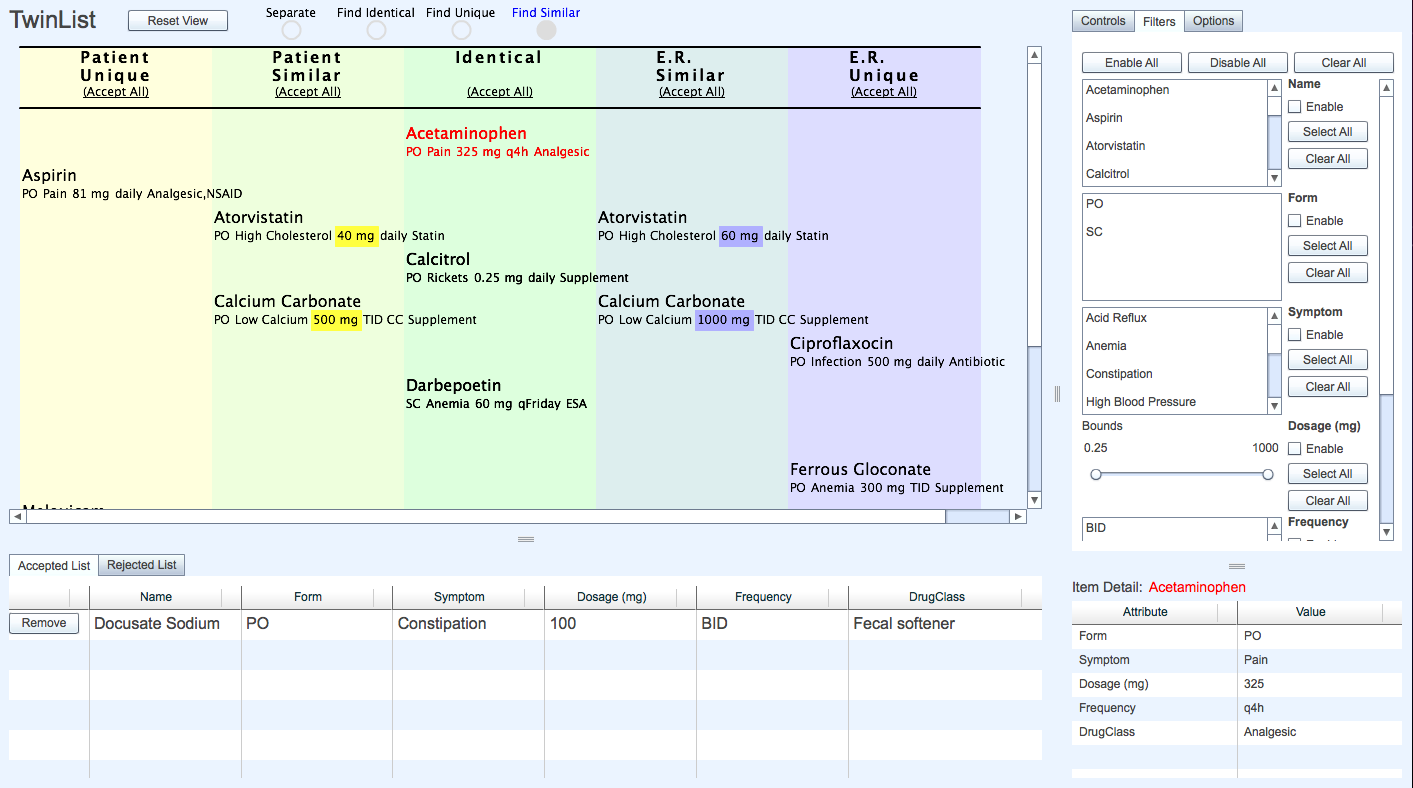
\includegraphics[width=1\linewidth]{img/interface2.png}
\end{center}
   \caption{The \TwinList~ interface: In this screen capture, the lists have been matched, displaying identical items in the center column, unique items in the outer columns and similar items in between. Color highlighting is used to indicate similar attribute values. In the bottom left panel is the \textit{Accepted} list; in the upper right panel, the \Filters; and in the lower right, the \Details, which displays all attributes for the selected item (highlighted in red).}
   \label{fig:interface}
\end{figure*}

\subsection{Related Work}
We explored multiple existing approaches for the design of \TwinList, though it seems that the specific problem of list comparison (as we have framed it) has seen relatively little research. Literature in areas such as visualizing text corpora and set membership are tangentially relevant in that they provide a basis for visualizing text similarity.  Collins et al. \cite{collins2009parallel} use tag clouds culled from text to compare several lists, using size to indicate frequency and giving a good overview of each document. Subsequent work extended this approach using spatial positioning, making it easier to find unique values \cite{conwaytuscon11}. The drawback of these approaches is that they are less useful in comparing specific list items, particularly when attributes must be considered.

Another well-researched area is set comparison. Venn Diagrams have long been used to illustrate intersection and symmetric difference. Kestler et al. \cite{kestler2005generalized} propose a modification allowing queries for a specific group of similarities and differences. While we prototyped a solution using Venn Diagrams, they ultimately did not fulfill the needs of our target applications.

Similarity matrices are well-suited to visualizing similarities between one item and multiple others \cite{CornelissenPCODA2007}. In addition, we developed a matrix-based visualization that would accommodate several lists. However, we dropped this approach, as the associated benefits were not likely to be relevant to our intended application domains, and it did not address attribute similarities.

Since attributes are of critical importance, we explored approaches that facilitate navigation through list attributes, such as \cite{Chimera:1992:VBI:142750.142817} and \cite{Masui98lensbar}. Ideas from each were incorporated into our initial designs, but were ultimately dropped as we focused on the core problem of list comparison.

Our decision to use animation was partly motivated by Chevalier et al. \cite{diffmation10}, in which animation and color are used to highlight the differences in document revisions. This naturally draws the user's gaze to the key areas needing attention. We incorporated these ideas into our design, feeling that animated transitions would make the process of list matching more interactive.

Our final design also incorporates the \textit{Eight Golden Rules of Interface Design} proposed by Shneiderman and Plaisant \cite{shneiderman}. Of particular interest were the principles of informative feedback and sequence closure.

Within the medical community, there has been much research \cite{JCAHO-2006} \cite{icutool03} highlighting the need for improved medication reconciliation. Preventable Adverse Drug Events (PADEs) are involved in 19\% of post-treatment complications. Trials of medication reconciliation policies show dramatic results. In one study, 94\% of patients had medication errors, of which a medication reconciliation process eliminated nearly all \cite{icutool03}. Although medication reconciliation has seen such  success, visualization tools for this procedure are still in their infancy. Our discussions with physicians suggested that many do not have adequate tools or a well-specified workflow for medication reconciliation. 

\section{TwinList}
\TwinList~ is a novel list visualization tool for the purpose of illustrating the similarities and differences between two lists. It can be used in many scenarios in which the comparison of two lists of items is required. The primary application that \TwinList~ supports is that of medication list reconciliation. However, \TwinList~ is equally adept in other applications, such as comparing bag-of-words lists or visualizing gene activity in brain tissue.

\TwinList's interface consists of four major components: the \ListViewer, \Tools, \AcceptedRejected~ lists and \Details, as shown in (Figure~\ref{fig:interface}). The \ListViewer, located in the upper left corner of the interface, is where the list matching visualization is performed. The initialized view displays two separated lists loaded from XML files. The \Tools, in the upper right corner, displays the \Controls, \Options~ and \Filters, which can be made visible one at a time by selecting the appropriate tab. If an item in the \ListViewer~ is selected, its detailed information is shown in the \Details, in the lower right corner. \TwinList~ is not merely meant for visualization; it also allows users to take action. List items can be accepted or rejected, whereupon they will appear in the \AcceptedRejected~ lists.

\subsection{ListViewer}
The  \ListViewer~ is the most important component in \TwinList's interface. It presents the two lists to be compared, using spatial placement and color to delineate identical, similar and unique items in the lists. Animated transitions are used to enhance understanding of these layout concepts, providing an interactive guide to the list comparison workflow.
%It is where the list matching animation and user actions are performed. The matching animation is triggered by pressing the \textit{Match List} button, or selecting any of the individual operations in the state diagram. The \ListViewer~ can be reset using the same button or state buttons.

\subsubsection{The five-column layout}
The five-column layout highlights the five possible outcomes of matching two list items. Each item is classified as being either unique to one list or identical/similar to an item in the opposite list. Identical items that occur in both lists are shown only once, and placed in the middle column. The extreme columns (one and five) contain items that are unique to a specific list. Items that are similar to one another are placed concurrently in columns two and four.

Each Item is rendered by its name string, with attributes below. To reduce clutter, the user may wish to select the attributes to render in the \ListViewer. This can be accomplished via the \AttributeFilter, located in the \Controls. The attributes that differ between similar items are highlighted to allow users to quickly identify discrepancies.

Color is used to provide a visual cue to the layout. The extreme columns have background colors yellow and slate blue, respectively. The middle column is the combination of these colors, green. Finally, the columns for similar items are yellow-green and blue-green, respectively. The color of the highlighting of similar attributes relates back to the color of each item's associated list. Pale background colors preserve the readability of the text. This palette does not pose problems for most colorblind users. By providing a constant visual cue to the user, we hope to ease the cognitive demand of identifying lists while matching.

To see the \ListViewer in action, refer to Figure~\ref{fig:interface}. Acetaminophen, Calcitrol and Darbepoetin appear on both lists, so they are placed in the center green column. Atorvistatin appears in both lists. However the dosage of the medication differs between the two lists, with 40mg on the patient list, and 60mg on the E.R. list. As a result, two instances of this item are shown in the second, yellow-green column and the fourth, blue-green column. The conflicting dosages are highlighted in the attribute text. Aspirin is unique to the patient list, so it is placed in the leftmost, yellow column.

\subsubsection{Matching Animation}
To emphasize the three stages of list matching, items move to their assigned columns through a sequence of animations, consisting of the following three steps:
\begin{enumerate}
\item The \Identical~ column header is rendered as the center background color fades in. Following this, identical items move into their respective locations in the center column.
\item The \Unique~ column headers and backgrounds are rendered similarly, after which unique items move into the first and last columns.
\item The \Similar~ column headers and backgrounds are rendered similarly, after which the similar items move vertically into their respective locations, as the previous animations may have changed the number of rows.
\end{enumerate}

The animation sequence can be viewed from start to finish via the \textit{Match Lists} button, or step-by-step via the animation states at the top of the \ListViewer, which act as button controls. After leaving the \textit{Separate} state, the \textit{Match Lists} button will become the \text{Reset View} button; clicking this will run the animation sequence backwards (from whichever state it happens to be in), thus reseting the visualization. The speed of the animation can be adjusted in relative increments via the \Options.

Figure~\ref{fig:animation} shows how the three stages of the list matching animation accentuate the \Identical, \Unique, and \Similar~ items at each step.

\begin{figure*}[t]
\begin{center}
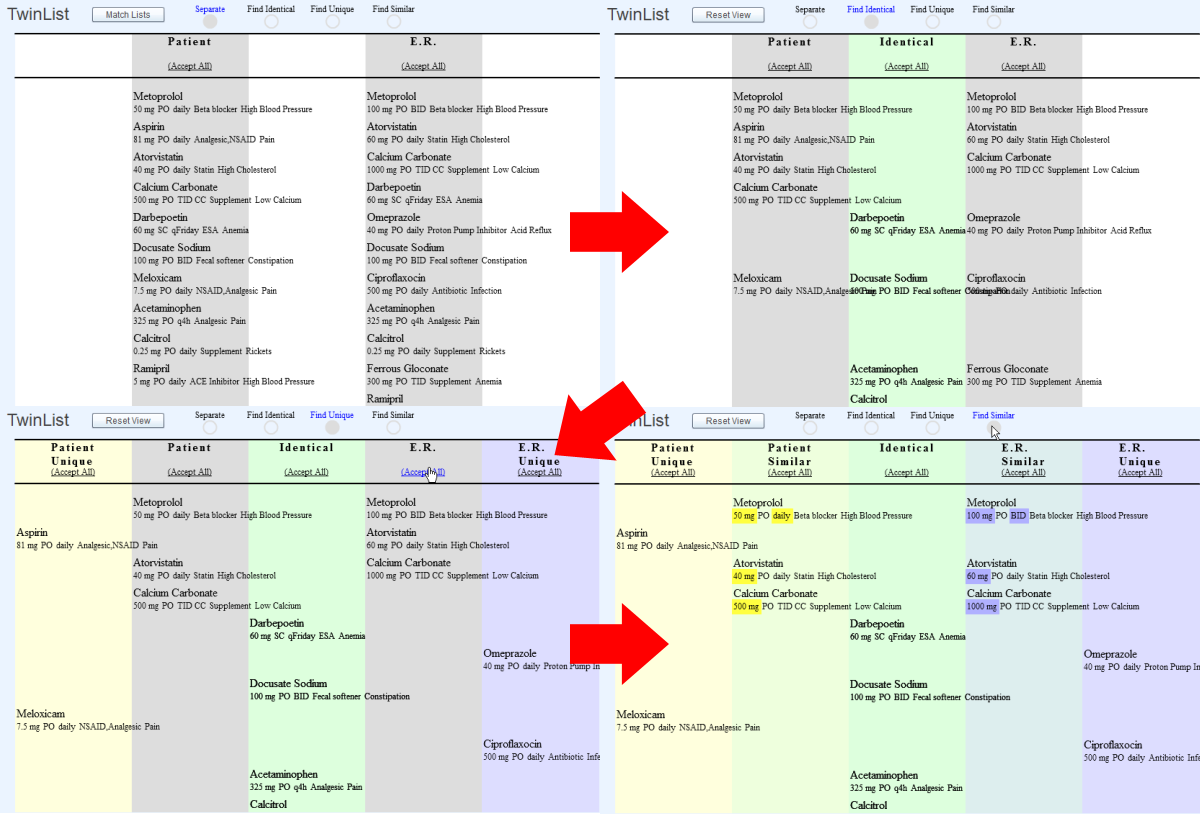
\includegraphics[width=1\linewidth]{img/anim_arrows.png}
\end{center}
   \caption{An animation sequence matching two lists of prescription drugs. The original \ListViewer~ is shown at the top left. In the top right, the \Identical~ items were found. The \Unique~ items are found next in the bottom left view. Finally, the \Similar~ items are matched with their differences highlighted in the bottom right view.}
   \label{fig:animation}
\end{figure*}

\subsubsection{Details on demand}
When the user clicks on an item, its information is shown in the \Details, illustrated in Figure~\ref{fig:details}. Although the user can choose to render every attribute value in the \ListViewer, the \Details~ provides details-on-demand when the \AttributeFilter~ is enabled.
%For example, a doctor can choose to only show the dosage, frequency and form of the medication and not to show drug class and symptom information, because they might be very familiar with most of the medications. They can still check the detail information on drug class and symptom in the  \Details~. We are not provide this feature in the current version.

\begin{figure}[t]
\begin{center}
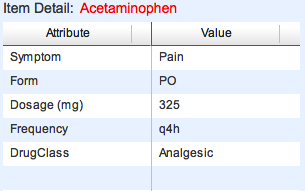
\includegraphics[width=1\linewidth]{img/details.png}
\end{center}
   \caption{\Details.}
   \label{fig:details}
\end{figure}

\subsubsection{Action taking}
After list matching is performed, the user should be able to clearly identify the similarities and differences between the two lists. While in certain applications, analysis alone may be sufficient, others may require the user to take action based on this information. This is especially useful in medication list reconciliation, in which the physician needs to decide which medications will remain in a patient's regime. \TwinList~ provides the functionality to accept or reject list items. When the user clicks and holds the left mouse button, a popup menu appears with the option to ``Accept" or ``Reject" (Figure~\ref{fig:menu}). While continuing to hold the left mouse button, the user positions the mouse over one of these options (which will become highlighted upon mouse-over) and then releases the mouse button to select. (Releasing the mouse button without selecting an option will simply close the popup without any action taken.)

Once the user has selected ``Accept" or ``Reject", the item is added to the top of either the \textit{Accepted} or \textit{Rejected} lists (Figure~\ref{fig:acceptlist}); the corresponding \ListViewer~ item is either removed or grayed-out, according to the user-configurable option (accessed in the \Options). Actions can be reversed by clicking on the ``Remove'' button next to each item in the \AcceptedRejected~ lists.

\begin{figure}[t]
\begin{center}
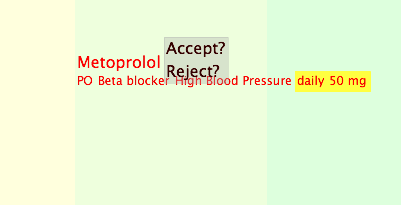
\includegraphics[width=1\linewidth]{img/menu.png}
\end{center}
   \caption{A detail of the action menu.}
   \label{fig:menu}
\end{figure}

\begin{figure}[t]
\begin{center}
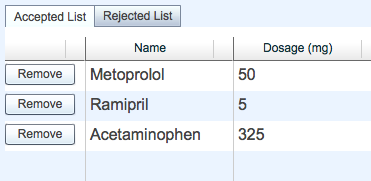
\includegraphics[width=1\linewidth]{img/acceptlist2.png}
\end{center}
   \caption{A detail of the \textit{Accepted} list.}
   \label{fig:acceptlist}
\end{figure}

\subsection{Controls}
The \Controls, depicted in Figure~\ref{fig:controls}, contains functionality for organizing and manipulating the the \ListViewer~ visualization. This includes the following components:
\begin{itemize}
\item \SizeBy: scales item text by its value for the given attribute. This control only works with numerical-type attributes.
\item \ColorBy: colors item text by its value for the given categorical attribute. This control only works with categorical-type attributes.
\item \GroupBy: organizes items by their values for the given attribute. This control works with either categorical- or general-type attributes (but not numerical).
\item \SortBy: sorts items (within groupings) by their values for the given attribute. This control works with any attribute. Note that the \GroupBy~ control has precedence over this control.
\end{itemize}
As of the submission of this paper, the \SizeBy~ and \ColorBy~ functionality is not operational, due to time constraints, though these features are planned for future iterations.

For an example of the usefulness of these features, consider the following scenario in the context of analyzing the State of the Union addresses. One might begin by grouping items (words) by their part of speech (assuming part of speech is an attribute). To further organize the display, one might then sort items by name (i.e. alphabetical ordering). The former lets the user analyze syntactical patterns, while the latter enables quick lookup of particular keywords. One can go even further, sizing words by their TF-IDF value, to reveal lexical patterns, similar to a Wordle\cite{Viegas2009}. In the context of medication list reconciliation, one might wish to group by drug class, size by dosage and color by frequency.
 
\begin{figure}[t]
\begin{center}
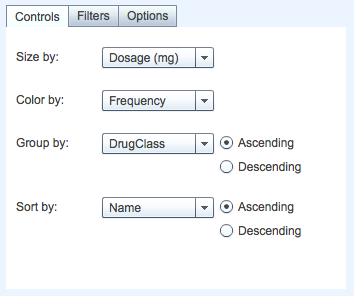
\includegraphics[width=1\linewidth]{img/controls.png}
\end{center}
   \caption{A detail of the \Controls.}
   \label{fig:controls}
\end{figure}

\subsection{Filters}
\TwinList's \Filters~ were inspired by those of Spotfire\cite{Ahlberg1996}. The ability to perform realtime queries and see the changes propagate to the visualization augments data exploration and analysis. For example, in medication list reconciliation, one might wish to display only certain drug classes, or only dosages in excess of a certain amount.\footnote{While in practice dosages are typically given on multiple scales --- e.g. 325 mg, 30 CCs --- we require that all numerical attribute values be normalized to the same scale.} Figure~\ref{fig:filters} depicts a detail of the \Filters.

Filters come in two classes: categorical and numerical. Categorical filters can be used to display only a specific set of attribute values, taken from a finite set of possible values. Numerical filters can be used to display only attribute values that fall within specified lower and upper bounds. Note that an item will only display it passes all filters, meaning its attribute values fall within the specified allowable sets or ranges.

A filter can be enabled and disabled via a checkbox displayed to the right of it. Enabling a filter implies that it is active. When a filter is disabled, it has no effect on the \ListViewer, no matter which values or bounds are set. The \textit{All} and \textit{None} buttons select or deselect all options in a categorical filter, where selection is demarcated by highlighting. A selected value is kept in the visualization. In a numerical filter, \textit{All} simply resets the bounds. The \textit{Reset All} button at the top of the \Filters~ resets all filters (though it does not disable them), equivalent to selecting \textit{All} on each.

\begin{figure}[t]
\begin{center}
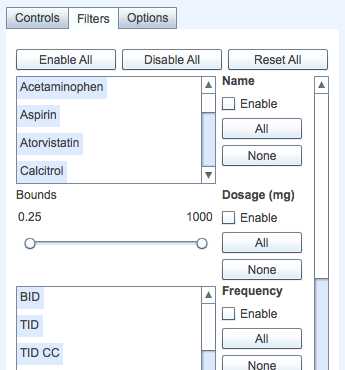
\includegraphics[width=1\linewidth]{img/filters2.png}
\end{center}
   \caption{A detail of the \Filters.}
   \label{fig:filters}
\end{figure}

\subsection{Options}
The \Options~ allows the user to control the following global application behavior:
\begin{itemize}
\item \textit{Dataset}: selects and loads a dataset from the three demo sets.\footnote{In future versions, the user will be allowed to upload a dataset using our proprietary XML schema.} Upon changing the dataset, the application will be reset, except for the \Options.
\item \textit{Font size}: sets the size of the font used to display item names in the \ListViewer. Note that the attribute text font size is relative to that of the name, though slightly smaller to reduce clutter.
\item \textit{Animation speed}: controls the relative speed of the animations in the \ListViewer. The speedup is defined as $2^\alpha$, where $\alpha$ is the slider value. Thus, a value of $\alpha = +1$ will double the speed and a value of $\alpha = -1$ will reduce it by $1/2$.
\item \textit{Link identical items}: determines how identical items are treated in the \ListViewer. When linked (the default), highlighting affects both items and accepting/rejecting either will hide the other from the \ListViewer. When unlinked, they are considered completely separate items.\footnote{Unlinking identical items implies that both items can be accepted or rejected, independent of the other.}
\item \textit{After item accept/reject}: determines the behavior of the \ListViewer~ after accepting or rejecting an item. \textit{Gray out} will simply gray the text and disable mouse actions; \textit{Remove} will hide the item from the \ListViewer.
\end{itemize}

\begin{figure}[t]
\begin{center}
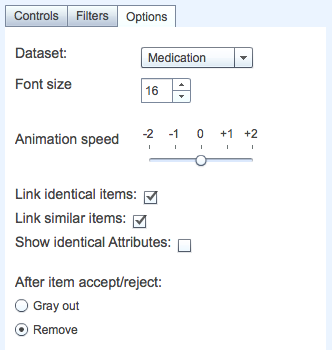
\includegraphics[width=1\linewidth]{img/options2.png}
\end{center}
   \caption{A detail of the \Options.}
   \label{fig:options}
\end{figure}

\section{Evaluation}
Our goal was to deliver a working prototype, not a finished, fully-functional application. As such, we were more concerned with qualitative rather than quantitative feedback on the features of our visualization system at this point. According to the categorization proposed by Lam et al~\cite{lam-bertini-isenberg-plaisant-carpendale-2011}, the evaluation scenario best matching our present purposes is the \textit{User Experience (UE)} test case. The goal of the following experiments was to observe how users reacted to the visualization and interactive features offered by \TwinList. We will use their feedback to improve the system's design in future versions.

\subsection{Experiment Design}
Test subjects came from two populations: two physicians and two graduate students in Computer Science (CS), both in the field of Human-Computer Interaction (HCI). The former used \TwinList~ to perform medication reconciliation. The latter was tested on the car data set (lists of features of two cars, one list per car). The testing protocol proceeded as follows: first, the user watched a $~7$-minute video demonstrating basic usage. Following this, the user was allowed to ask questions. Next, the user interacted with the system unaided, performing either specific tasks (medication reconciliation case studies) or general, free exploration ones (car data case studies). While using the system, subjects were encouraged to \textit{think aloud}~\cite{lewis-1982}. The entire experiment was recorded in both audio and screen capture video. 

\subsection{Case 1: Med. reconciliation, A. Z. H., male, 34 y. o.}
Overall, the participant performed the tasks as expected and reported anticipated results. A. Z. H. purported to be very comfortable with computers. He does not perform medication reconciliation on a regular basis, except when doing inpatient aid and discharge from the hospital, for which he does not use any software. This is how he describes his \TwinList~ experience: \textit{``It's really impressive, the way you organize things is great. It's definitely a step in the right direction \dots"}. He was very enthusiastic and provided several suggestions, most of all worth including in this section. 

\subsubsection{Results}
The following notes summarize A. Z. H.'s experience:
\begin{itemize}
\item There is need for an indication that there are more items than what can be currently seen in a column. The scroll bar alone is insufficient.
\item It is difficult to get to the \AcceptReject~pop-up menu when accepting/rejecting an item. He had trouble with the click-and-hold behavior, wanting instead to use the mouse's right-click button.
\item To send items from \AcceptedRejected~lists back to the viewer one-by-one requires quite some effort when you have many items in those lists. A \textit{Remove All} button would be desirable.
\item Warning dialogs or undo may be needed when accepting and rejecting items, since it is a delicate operation in medication reconciliation.
\item In the control panel, drop-down boxes should indicate what the default \GroupBy/\SortBy~attributes are, instead of blank captions. (The default is actually the original ordering.)
\item It would be desirable to shorten vertical empty spaces in between items to minimize the need of scrolling.
\item The number of visible item attributes should be shortened in the \ListViewer, since reconciliation is performed, in practice, based on only a few (e. g. the \textit{Indication} feature).
\item For items in the \Similar~columns, the item pop-up menu should have a third option, to automatically reject an item of a list if its counterpart at the other list was accepted. According to the participant, this would be the likely outcome in almost every such context.
\item The participant suggested that we should change the way items are displayed so that, for each list, you have items sorted by some \textit{uniqueness level}; for example, by vertically ranging from identical to unique. This would add more meaning to the vertical structure of the list, which is somewhat lost after lists are matched, but would represent a significant change in the concept.
\item The participant felt that placing the \AcceptedRejected~lists at the bottom of the interface may be suboptimal for tracking what happened to processed items, especially when the user gets distracted.
\item The participant missed being able to interact on the spot with accepted/rejected items that are grayed out. In his words: \textit{``If it is grayed out, what if (\dots) I really want to do the 100 mg, is there any way to click and have it re-instate (\dots) or un-reject/un-accept"}. He believes that if he could interact with grayed-out items on the viewer, the \AcceptedRejected~lists might not even be necessary, thus allowing more room for the main visualization. As such, the list of rejected/accepted items could be output as the final product of the interactive process and would be activated by pressing a button. As he suggested: \textit{``\dots Here is your final list of medications, this is your rejected list over here, and when one finally accepts, export to (\dots) or put in patient's medical record \dots"}.
\item The participant suggested an additional \SortBy~criteria: in his own words, \textit{``medications that haven't been dealt with yet."} We translate this as a grouping of medications based on their accepted/rejected status. This is a useful, general concept applicable to other list matching problems.
\item The participant mentioned the importance of filters, especially to filter by route (e.g. I.V. medications).  
\end{itemize}

\subsection{Case 2: Med. reconciliation, M. G., male, 62 y. o.}

Unlike the previous participant, M. G. had more trouble performing his tasks. His reactions clearly indicated that he expected the system's terminology to be geared more towards medication list reconciliation
%(such as having \textit{Match Lists} as the caption of the button that triggers list matching, instead of \textit{Reconcile Lists})
than general list matching. As the matching animation began, he expressed feeling overwhelmed: \textit{``Wow, what just happened there?"}. M. G. considers computers somewhat hard to use (he reported a difficulty score of 4 out of 5). This subject performs medication reconciliation every day. 

\subsubsection{Results}
The following notes summarize M. G.'s experience:
\begin{itemize}
\item In his opinion, one item's list of attributes should not exceed the width of its column. He felt that the piece of the attribute list that spills into the next column could be associated with another item in that column, which could lead to a serious confusion: as he pointed out, the dosage of one medication could be mistakenly associated with another item.
\item The participant became confused by the step-wise animation buttons when told to accept all identical items. When asked to accept all identical items, he clicked  \textit{Find Identical} instead of \textit{Accept All}. The animation then proceeded half-way through and he realized his mistake. He tried to fix it and ended up clicking on \textit{Find Unique}. Finally, when he tried to accept/reject items, he realized that similar items across both lists were not in the same row of the viewer. The reason was that he had not completed the list matching animation. This indicates that the list matching should be performed as an atomic operation, instead of allowing the user to step through the stages. (This is perhaps supported by the fact that the first physician never even touched the step-wise matching feature.)
\item An unexpected outcome of this test was that the participant somewhat associated temporal order from left to right, as if the first list represented an event that necessarily came before the second list. He compared the dosage of the drugs at the Patient's \Similar~ column (left) with the corresponding drugs/dosages at the E.R. column (right), and tried to infer some sort of temporal pattern regarding how the patient was dealt with in the E.R.: \textit{``Conceptually, I think it is a nice setup, actually, because you can try to deduce what went on during the stay in the E. R. For these drugs, they decided that the patient needed more of that, because they increased the dose ..."}. Although this was not the intent of the synthetic data, nor the visualization, to associate temporal meaning to the visualization might be an interesting path to explore in the future.
\item The issue of having to unnecessarily reject a similar item after accepting its counterpart appeared again, particularly if dosage is the single attribute that changed across items: \textit{``If it is absolutely the same in every respect, except for the dosage amounts, you can't give two dosage amounts simultaneously ..."}. (Note: this feature has been added in the most recent version.)
%\item Unlike the other participating physician, M. G.  thought that \textit{Indication} is not a very descriptive attribute since a drug can be prescribed for several reasons. On the other hand, he likes the \textit{Drug Class} feature and, after being asked about it, he agrees it could be a useful feature to group by.
\end{itemize}

\subsection{Cases 3 and 4: Car data, T. L., male / A. N. S., female.}

Both participants are doctoral student in CS/HCI. In particular, the first one has a background in interactive design and is very familiar with usability testing. T. L. had trouble to grasp the list matching idea at first, but after some explanation and background information he understood the concept well. He had very few problems while interacting with \TwinList, and was particularly impressed with the animation. A. N. S. performed the experiment very smoothly and had no problem interpreting the visualization. She immediately came up with a plan on how to find similar items and detect differences, clearly describing the steps she took to reach her results. A minor difficulty she encountered was to operate the \AcceptReject~ pop-up menu. In fact, it is a recurring problem, since it also happened to the first participant in the medication list reconciliation experiment. However, after A. N. S. was reminded on how to operate the feature, she was quickly able to make it work. 

\subsubsection{Results}
The most prominent insights from these experiments were:
\begin{itemize}
\item T. L. complained about the size of the \ListViewer. This brings back some suggestions of participant A. Z. H., who pointed to the lack of ``vertical meaning" after matching is performed. In fact, when items are removed from the viewer, the panel is left with apparently unnecessary, empty rows, potentially increasing the need of vertical scrolling. 
\item To perform list matching, T. L. seemed to prefer the step-wise matching buttons to the \textit{Match Lists} button on the left. We believe this was mostly due to the exploratory nature of this particular experiment, that the participant was encouraged to explore the interface as thoroughly as possible.
%\item While exploring the filters, A. N. S. was confused by the attribute descriptions in the drop down menu. To her, terms such as ``priority ()" would appear more as a function call rather than an attribute name. She suggested that we should use more understandable wording for the attributes during the preprocessing the data.
\item A. N. S. was very impressed with the filter options but did not like the fact that the viewer changes size after filtering. This is a side-effect of the automatic sizing that could be removed in future iterations.
\end{itemize}


\section{Conclusions and Further Directions}
Our goal was to create a list comparison tool to assist list matching for many applications, with a particular focus on medication list reconciliation. We designed an intuitive spacial organization for differentiating identical and unique items, as well as highlighting the differences in similar items. The use of animation reinforces the user's understanding of this layout and emphasizes the procedural aspect of list matching. The included filtering, grouping and sorting tools allow the user to thoroughly explore a dataset.

By conducting a number of case studies, we gained additional insights about the design and use of this tool. Evaluation results revealed that testing subjects from both populations were positively impressed with the tool and supported our expectations. From the medication list reconciliation results, we can say that both users approved of our five-column layout and color-coded highlighting (attribute-based differences), two key concepts behind \TwinList. We also learned that the step-wise list matching feature appears to be superfluous and potentially troubling, suggesting that list matching, both from the procedural and visual perspective, should be performed as an atomic sequence. The exploratory experiments performed with CS/HCI students revealed some flaws in our interface designs, from use of vertical space to difficulties with the input controls. All of these comments will be taken into consideration as development moves forward on \TwinList.
 

\bibliographystyle{abbrv}
\bibliography{twinlist}

\end{document}
